\documentclass[12pt]{article}
%Gummi|065|=)
\usepackage{amsmath, amsfonts, amssymb}
\usepackage[margin=0.5in]{geometry}
\usepackage{xcolor}
\usepackage{graphicx}

%\usepackage{pifont}
\usepackage{amsmath}



\newcommand{\off}[1]{}
\DeclareMathSizes{20}{30}{20}{18}

\newcommand{\two }{\sqrt[3]{2}}
\newcommand{\four}{\sqrt[3]{4}}
\newcommand{\red}{\begin{tikz}[scale=0.25]
\draw[fill=red, color=red] (0,0)--(1,0)--(1,1)--(0,1)--cycle;\end{tikz}}
\newcommand{\blue}{\begin{tikz}[scale=0.25]
\draw[fill=blue, color=blue] (0,0)--(1,0)--(1,1)--(0,1)--cycle;\end{tikz}}
\newcommand{\green}{\begin{tikz}[scale=0.25]
\draw[fill=green, color=green] (0,0)--(1,0)--(1,1)--(0,1)--cycle;\end{tikz}}

\newcommand{\sq}[3]{\draw[#3] (#1,#2)--(#1+1,#2)--(#1+1,#2+1)--(#1,#2+1)--cycle;}

\usepackage{tikz}
\usetikzlibrary{arrows}
\usetikzlibrary{decorations.markings}

\newcommand{\susy}{{\bf Q}}
\newcommand{\RV}{{\text{R}_\text{V}}}

\title{Scratchwork: Box Counting}
\date{}
\begin{document}

%\fontfamily{qag}\selectfont \fontsize{12.5}{15}\selectfont

\sffamily

\maketitle

\noindent Here's a nice question about Counting Boxes: \\ \\
The number of plane partitions that fit inside an $a \times b \times c$ box is:
$$ M(a,b,c) = \prod_{i=1}^a  \prod_{j=1}^b  \prod_{k=1}^c \frac{i+j+k-2}{i+j+k-1}  = \frac{H(a)H(b)H(c)H(a+b+c)}{H(a+b)H(b+c)H(c+a)}$$
where $H(a) = 1! \,2! \,3!\, \dots \,a!$ is the \textbf{hyperfactorial}. \\ \\
In this branch of math, almost any enumerative question you can think of has been 
discussed and generalized several times over. The notation may be clumsy and difficult 
to read, but there is always an answer.  This is true, because the boxes have a very very large symmetry attached to them, that we can use at any time.  This algebra, at least the size of $\widehat{\mathfrak{gl}}(\infty)$. \\ \\
Like all branches of mathematics, there degrees of specialization and many points of view.  \\ 
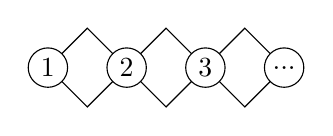
\begin{tikzpicture}
\draw[->] (0,0) -- (0.5, 0.5) --(1,0);
\draw[->] (0,0) -- (0.5,-0.5) --(1,0);
\draw[fill=white] (0,0) circle (0.25);
\node (1) at (0,0) {1};
\draw[->] (1,0) -- (1.5, 0.5) --(2,0);
\draw[->] (1,0) -- (1.5,-0.5) --(2,0);
\draw[fill=white] (1,0) circle (0.25);
\node (2) at (1,0) {2};
\draw[->] (2,0) -- (2.5, 0.5) --(3,0);
\draw[->] (2,0) -- (2.5,-0.5) --(3,0);
\draw[fill=white] (2,0) circle (0.25);
\node (3) at (2,0) {3};
\draw[fill=white] (3,0) circle (0.25);
\node (4) at (3,0) {...};
\end{tikzpicture} \\ 
Given, there is so much activity on one part of the board, we can just assume there is going to be generalizatino there.  Where could we play instead? \\ \\
\includegraphics[width=6in]{boxes-02.png} 

\includegraphics[width=6in]{boxes-01.png} 



\vfill

\begin{thebibliography}{}

\item MathOverflow \textbf{Why does McMahon formula look like the inclusion-exclusion principle?} \texttt{https://mathoverflow.net/q/219073/1358}

\item Alexei Borodin, Vadim Gorin \textbf{Shuffling algorithm for boxed plane partitions} \texttt{arXiv:0804.3071}

\end{thebibliography}



\end{document}